\chapter{Determination of the material budget}
\label{chap:X0}

  The discovery of new physics and the characterisation of the already known particles are possible only with performant detectors.
  As it was presented in chapter~\ref{chap:vxd}, the fabrication of a vertex detector is mostly constrained by two parameters: the pointing resolution and the material budget.
  The first fully functional prototype of \gls{PLUME} was tested in November 2011 at CERN with 120 GeV pions.
  The results have shown that the pointing resolution of the ladder corresponds to the expected value for the \gls{ILD}.
  Moreover, the use of a double-sided structure improves this pointing resolution. 
  Nevertheless, the material budget ($\rm{X_0}$) of \gls{PLUME} has not been studied yet and only estimated by calculation.
  SPS beam is involving particles with too high momentum, so they suffer less from the effect of the multiple scattering.
  %Nevertheless, the material budget ($\rm{X}_0$) of such device is estimated only by calculation and the SPS beam is involving particles with too high momentum that are not suited to perform this measurement.
  Therefore, a test beam campaign of the PLUME-V1 prototype was done in April 2016 at DESY test beam 21 with positrons up to $5~\rm{GeV}$.
  Firstly, the presentation of the test beam is discussed.
  Secondly, the motivation, the test beam facility, as well as the tools used for the analysis are presented.
  Finally, the last section is dedicated to the data analysis leading to the radiation length measurement.

\minitoc

  \section{Preparation of the test beam}

  In April 2016, a test beam campaign with electrons up to 5 GeV was performed at the DESY-II test beam facility \cite{DESYII}.
  The preparation of a test beam campaign is a long, intense and stressing period.
  The different aspects of the test beam have to be carefully thought to minimise the problems and the time spent for debugging during the test period.
  This consists in scheduling precisely the different measurements that have to be performed during the restricted time, as well as the set-up to use, the integration of the \gls{DUT} and the acquisition system to use.
  
    \subsection{Measurements and telescope configuration}

    Although the first prototype was validated with $120~\rm{GeV}$ pions in November 2011 at CERN, two aspects were not yet studied.
    The first one is the ability of the detector to detect and track low momentum particles such as electrons.
    The spatial resolution, the detection efficiency and the benefits of mini-vectors with the DESY test beam have to be measured and compared to the values obtained at CERN.
    Runs with different tilts (from $0^{\degree}$ to $60^{\degree}$ with a step of $10^{\degree}$) and different air flow speeds for the cooling system ($3~\rm{and}~6~\rm{m.s}^{-1}$) are performed to study again the mechanical deformations of the ladder.
    The second aspect not yet studied is the measurement of the equivalent radiation length of \gls{PLUME}.
    For the first time, the collaboration wants to confirm the theoretical estimations, which give a weighted material budget $\left. \rm{X_{0}}\right|_{\rm{weighted}} \simeq 0.65~\%$ for the version tested.
    Although many runs were acquired to perform the different measurements, the test beam was scheduled at the end of my Ph. D.
    Therefore, I am not able to perform a complete analysis of the first prototype for low momentum electrons.
    Section~\ref{sec:X0} presents the study I have performed on the radiation length measurement.

    Before going to the test beam and acquiring data, the geometry of the telescope has to be determined to optimise the tracking.
    This depends on the spacing between the different planes and the position of the \gls{DUT} respectively to the telescope.
    The best track extrpolated on the \gls{DUT} position is achieved by placing the inner planes of the telescope as close as possible to the \gls{DUT} and the outer planes as far as possible from the \gls{DUT}.
    Because of the deformation study, which needs to rotate the ladder (see chapter~\ref{chap:deformation}), the inner planes can not be pressed to the \gls{DUT} without modifying the geometry at each steps.
    Hence, to keep a consistent alignment and to reduce the time spending on the off-line alignment, it was decided to fix the inner planes as close as possible to be able to rotate the ladder without modifying the geometry.
    Moreover the ladder is not centered in its box, so to keep an equal distance between the two sides of the ladder and the two inner planes, the minimal distance between the telescope planes are calculated by taking into account an offset.
    It has to be noted also, that for the radiation length measurement, the geometry is different.
    The upstream planes are stacked together and really close to the \gls{DUT}, whereas the downstream planes are distant from each other.

    For the first time, the collaboration has decided to use the EUDET telescope and EUDAQ \cite{EUDAQ} for the acquisition, instead of the Strasbourg telescope and the IPHC acquisition.
    Several configuration are available for the set-up used.
    The first ones consist to use the six planes of the EUDET telescope \cite{Jansen} and to have two separate acquisitions, one for \gls{PLUME} and the second one dedicated for the telescope.
    Then, the data have to be merged together.
    As the EUDET telescope is equipped with the same sensors as \gls{PLUME}, the acquisition can be simplified by having only four telescope planes and connecting directly two sensors of the \gls{DUT}.
    A simulation toolkit developed by Simon \textsc{Spannagel} \cite{spannagel_2016_48795} and based on \gls{GBL} \cite{GBL} is used to compare the pointing resolution at the \gls{DUT} position for different telescope geometries.
    Here, the six and four telescope planes set-ups are compared for different energies and spacing between the sensors.
    This simulation takes into account the material budget of the telescope, the \gls{DUT} and the multiple scattering of electrons in the air\footnote{The simulation is not based on a proper Monte-Carlo tool, but calculates the multiple scattering with an approximation of a Gaussian process}.
    One telescope plane has a material budget of $\sim 0.053~\%$ of $\rm{X_{0}}$, whereas \gls{PLUME} is $\sim 0.65~\%$ plus two kapton foils used to insulate the ladder from the light ($\sim 0.071~\%~\rm{X_{0}}$).
    For both configurations, the telescope is divided into two arms, two or three planes on each side of the \gls{DUT}.
    The maximal distance between each reference plane of one frame is $\rm{d}_{\rm{max}} = 150~\rm{mm}$ for the six sensors configuration, whereas for the second one it is $\rm{d}_{\rm{max}} = 300~\rm{mm}$.
    
    \begin{table}[!h]
      \centering
      \begin{tabular}{c c c}
        \hline %----------------------------
        \multirow{2}*{Energy (GeV)} &  \multicolumn{2}{ c }{$\sigma_{\rm{res}}~\rm{(\mu m)}$} \tabularnewline
                              &  4 planes & 6 planes \tabularnewline
        \hline %----------------------------
        \hline %----------------------------
        2 & 4.9 & 4.8 \tabularnewline
        3 & 3.8 & 3.8 \tabularnewline
        4 & 3.4 & 3.4 \tabularnewline
        5 & 3.1 & 3.2 \tabularnewline
        6 & 3.0 & 3.0 \tabularnewline
        \hline %----------------------------
      \end{tabular}
      \caption{Estimation of the resolution on the track extrapolation $\sigma_{\rm{res}}$ at the DUT position for a telescope with four planes and six planes. Practical issues, such as the alignment, will limit the precision on the track extrapolation to $100~\rm{nm}$.}
      \label{tab:estimationRes}
    \end{table}

    Table~\ref{tab:estimationRes} summarises the resolution on the track extrapolation at the \gls{DUT} position for different energies and the use of four or six telescope planes does not have an impact on the telescope pointing resolution.
    Figure~\ref{fig:estimationRes4.7GeV} displays the pointing resolution as a function of the different spacing between two telescope planes of the same frame, for an energy sets to $4.7~\rm{GeV}$.

    \begin{figure}[!b]
      \centering
      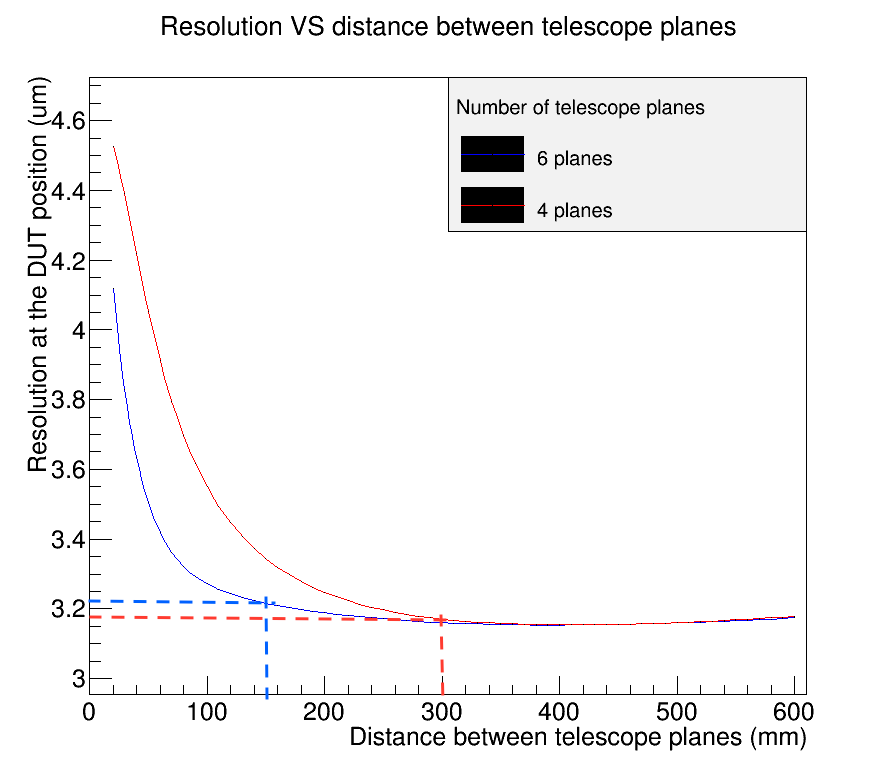
\includegraphics[width = 0.7\textwidth]{Pictures/X0/resolution_4Vs6planes_4-7GeV.png}
      \caption{Estimation of the track extrapolation resolution at the DUT position as a function of the distance between two telescope planes of the same arm for an energy of $4.7~\rm{GeV}$.
      The blue lines is the results for six planes, whereas the red line is for four planes. 
      The dashed lines are the maximal distance between two planes due to the rail limitation of the telescope frame.}
      \label{fig:estimationRes4.7GeV}
    \end{figure}

    As the number of telescope planes does not impact the pointing resolution, it has been decided to use only four telescope planes and two \gls{PLUME} sensors (one on each side) to simplify the acquisition system.
    However, the synchronisation and the stability of the acquisition have to be tested before the test beam campaign. 

    \subsection{Acquisition system and experimental set-up}
      
      \subsubsection{EUDAQ}

      EUDAQ is a modular cross-platform data taking framework developed for the EUDET-type beam telescopes \cite{Jansen}.
      It is designed to be flexible and to have an easy integration of other devices.
      The software is based on \textit{producers}, that are linked between the different subdetector systems, such as the beam telescope, the \gls{DUT} user's DAQ and the \gls{TLU} \cite{Cussans2009}.
      The events of each subdetector are then correlated to form one single global event for data belonging to one trigger.
      This step is done by the \textit{Data Collector}.
      The robustness of the acquisition set-up planed is tested by performing multiple runs for multiple configuration in the laboratory.
      The data are acquired with only the \gls{PLUME} to ensure that EUDAQ can cope it, and then single \gls{MIMOSA}-26 sensors are added and runs of several hours are performed to look for a loss of synchronisation.

      \subsubsection{Experimental set-up}

      Finally, the integration of \gls{PLUME} for the different measurements to perform is investigated.
      For the deformation studies, the \gls{DUT} is mounted on a rotation stage. 
      With respect to the local coordinate system (or sensor coordinate system), the rotation is along the $u$-direction. 
      The first option considered to perform the rotation is to orient the ladder in the same direction as the telescope's sensors. 
      Hence, the ladder is in the horizontal position and the rotation needs a complicated frame to ensure the stability of the system.
      The weight of the box and ladder is applied only on the rotation stage. 
      Due to the complexity and the time needed to build this frame, a second option has been considered.
      The ladder is placed vertically on a rotation stage. 
      There is a $90^{\circ}$ rotation between the telescope sensors and the \gls{PLUME} ones.
      The frame consists of an insulated aluminum plate on which the \gls{DUT} sits.
      To avoid damaging the \gls{DUT} during the test beam, the flex-cable is maintained on the frame by two clamps.
      In this way, less constraint are applied on the connectors. 
      A plate with screws hold the ladder strongly to the frame.
      The frame is then mounted onto a rotation stage, which is mounted on a translation stage.
      Figure~\ref{fig:mechanics} shows a schematic model of the frame designed and built at DESY.
      
      \begin{figure}[!b]
        \centering
        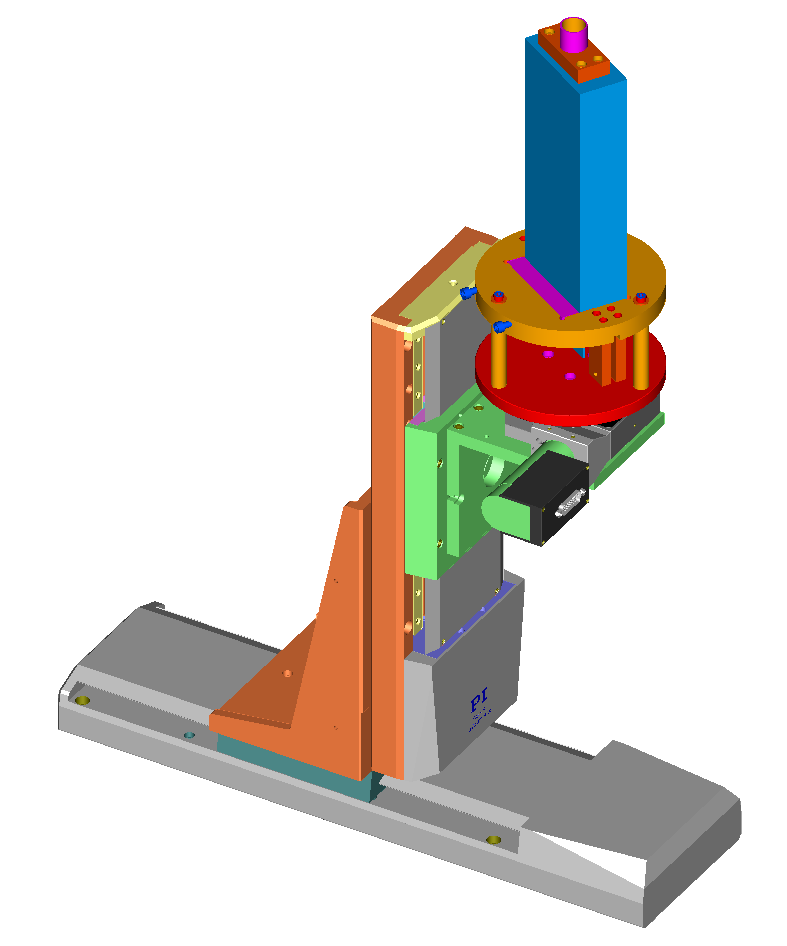
\includegraphics[width = 0.5\textwidth]{Pictures/X0/Frame/Testbeam1.PNG}
        \caption{TCAD model of the mechanical structure designed for the test beam in April. The ladder is hold on a circular frame fixed to a PI rotation stage, mounted onto a XY-table.}
        \label{fig:mechanics}
      \end{figure}

      To control the heating of the ladder during the test beam, a cooling system consisting of a simple fan is used.
      On one endcap, a pipe is fixed and connected to the fan.
      Some studies in Strasbourg were done to determine the air flow speed as a function of the voltage applied.
      Hence, an air flow speed of $3~\rm{m.s^{-1}}$ is achieved with $5~\rm{V}$ and an air flow speed of $6~\rm{m.s^{-1}}$ for $10~\rm{V}$.
      This values result in an operating temperature of all sensors between approximately $40^{\degree}\rm{C}$ and $52^{\degree}\rm{C}$.

      During the test beam campaign, the \textit{clock} and \textit{marker} are read from one sensor of \gls{PLUME}.
      The \textit{clock} is extended with a $80~\rm{cm}$ long cable to ensure that one frame starts on the rising edge.
      The second input of the acquisition is a \gls{PLUME} sensor (opposite side of the first sensor), followed by the four telescope planes. 
      Moreover, \gls{PMT}s are placed in coincidence on each side of the telescope.
      They are used to trigger the acquisition only when the beam passes through the entire set-up.
      Hence, the fake events are reduced and the data stream is smaller.
      Figure~\ref{fig:testBeamAcq} shows a schematic of the acquisition and set-up used during the test beam, while figure~\ref{fig:testBeam} is a picture of the system taken during the test beam.

    \begin{figure}[!h]
      \centering
      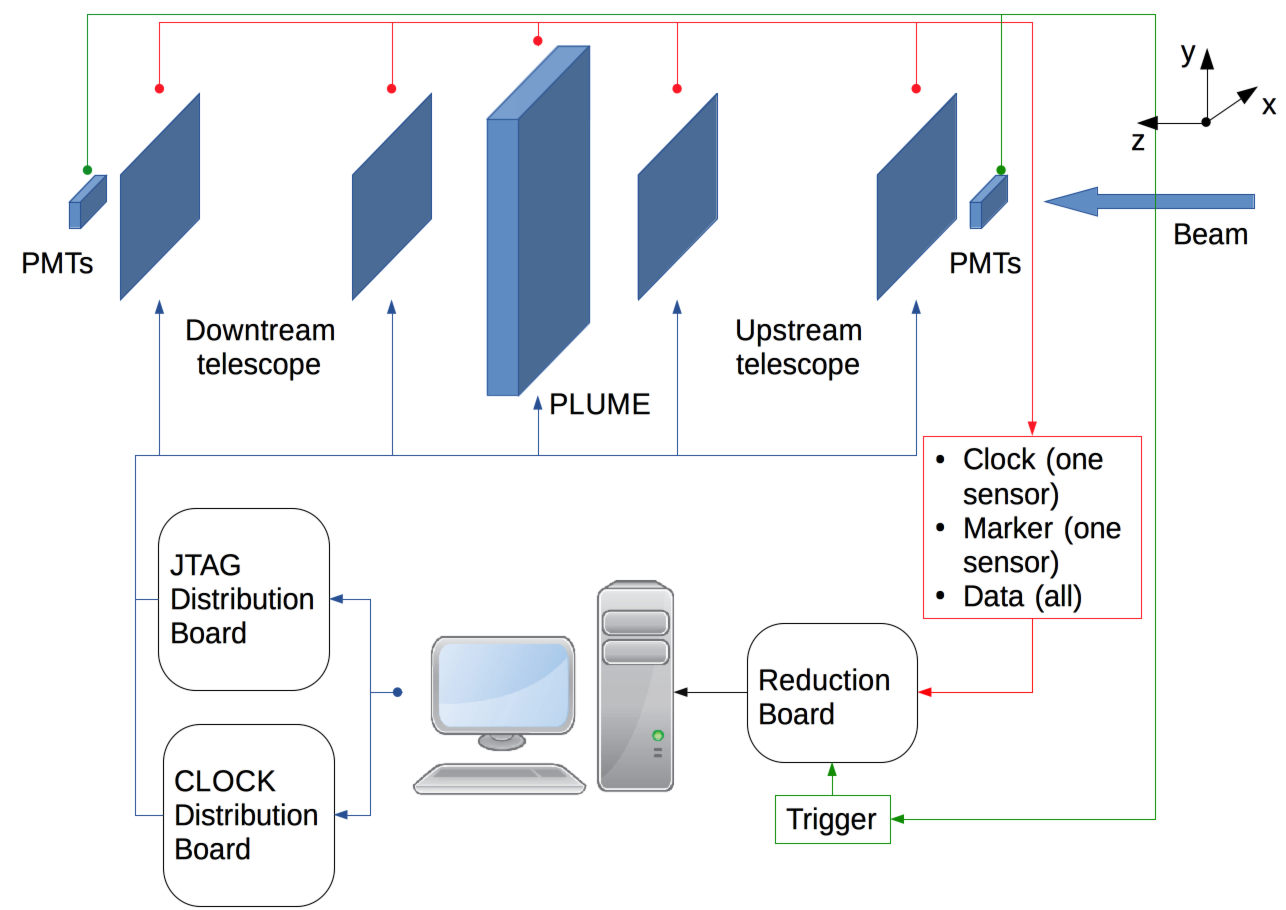
\includegraphics[width = \textwidth]{Pictures/X0/testBeamAcquisition.png}
      \caption{Schematic of the test beam set-up. The PMTs are used for triggering. The clock and marker are read from only one sensor, here it comes from one PLUME sensor.}
      \label{fig:testBeamAcq}
    \end{figure}

    \begin{figure}
      \centering
      \includegraphics[width = 0.8\textwidth]{Pictures/X0/testBeam.png}
      \caption{Picture taken during the test beam. The beam is going out of the magnet (large red frame) before reaching the four detection planes (aluminum square frames), the DUT (elongated box) and the PMTs (one is visible at the left-end of the picture). The set-up is mounted on a floating frame insuring the electrical grounding.}
      \label{fig:testBeam}
    \end{figure}

    \subsection{Issues during the test beam}

    The preparation of the test beam, as well as the data taking were a long and stressful period.
    Although everything were prepared as mush as possible to avoid any problem during the test beam, a broken component on the power distribution board has disturbed the data taking for two days.
    One \gls{PLUME} module was not recording data anymore but was still sending \textit{header} and \textit{trailer}.
    Fortunately, after replacing the broken component, the ladder was working normally, but a shift on the thresholds has appeared.
    By characterising again the ladder, it has been possible to determine which thresholds were really applied. 
    Nevertheless, it is likely that some data could have been corrupted and this is under investigation.
   
  \section{Measuring the radiation length}

    \subsection{Introduction}
    
    When charged particles are traveling through matter, they lose energy via inelastic collisions with atomic electrons and this leads to the ionisation or excitation of the matter.
    Furthermore, along their path, they are deflected by many small angles from their initial trajectory due to Coulomb scattering from nuclei. 
    This stochastic effect, called multiple Coulomb scattering, leaves on the average the particle undisturbed through its path. 
    For small angles of deviation, the multiple scattering is following a Gaussian behavior, whereas for larger angles, it behaves like the Rutherford scattering.
    The Highland formula, which is an empirical formula, describes the distribution of the multiple scattering, or the "kink angle" $\theta_0$ as a function of the momentum $p$ of the incoming charge particles, its velocity $\beta c$, its charge number $z$ and its true path length in radiation length unit $\frac{x}{X_{0}}$:

    \begin{equation}
      \theta_{0} = \frac{13.6~\rm{MeV}}{\beta c p}\cdot z \cdot \sqrt{\frac{x}{X_{0}}}\left(1 + 0.038 \cdot \ln{\left(\frac{x}{X_{0}}\right)}\right).
      \label{eq:Highland}
    \end{equation}

    For the electrons, a modified version of the equation~\ref{eq:Highland} describes its scattering better than the Highland formula does \cite{GEANT4}.

    \begin{equation}
      \theta_{0} = \frac{13.6~\rm{MeV}}{p}\left(\frac{x}{X_{0}}\right)^{0.555},~\text{with $\beta c = 1$.}
      \label{eq:theta0}
    \end{equation}

    The spread angle $\theta_{0}$ depends on the momentum of the incoming particle, as well as the relative radiation length $\frac{x}{X_{0}}$.
    Thus, for a given relative radiation length, the kink angle is becoming smaller for higher momentum.
    %The kink angle is also different depending on the relative radiation length for a given momentum. 

    It is possible to determine the radiation length $\rm{X_0}$ of a material knowing the energy of the particle, its thickness $x$ and by measuring the kink angle $\theta_0$.

    \subsection{Motivation}

    The design of a detector is driven by its intrinsic characteristics, such as the pointing resolution or the integration time, but also by some requirements on the material budget.
    For example, the \gls{ILC} sets new goals for the design of the vertex detector, but also for other parts of the detector, as mentioned in chapters~\ref{chap:ILC} and~\ref{chap:vxd}.
    For such detector, the tracking system should detect precisely the particles path and minimise their energy degradation, while the calorimeters have to measure accurately the energy deposited by the particles.
    During the physics analysis, the reconstruction of the events depends strongly on the knowledge of the energy loss by the particles inside the different components of the detector before they reach the calorimeters. 
    To improve the results, a correction on the energy has to be applied.
    Thus, the study of the radiation length $\rm{X_{0}}$ in $\rm{g.cm}^{2}$, which is the amount of matter traversed by the electron is an important part of the detector development.
    For electrons and positrons, the radiation length corresponds to the mean distance over which these particles loss $1/e$ of their energy by bremsstrahlung.

    As detector are made of different layers, the radiation length for composite materials is given as:

    \begin{equation}
      \frac{1}{X_{0}} = \sum_{j} \frac{\omega_{j}}{X_{j}},
    \end{equation}

   where $\omega_{j}$ and $X_{j}$ are respectively the fraction by weight and radiation length for the $j^{\rm{th}}$ element.

    \subsection{The DESY II test beam facility}

    The \gls{DESY} test beam facility \cite{DESYII} is composed of three areas.
    The electron beam is produced in the LINAC-II and accelerated up to 450 MeV before to be injected in the DESY-II synchrotron ring.
    The DESY-II is used as a storage ring for the PETRA-III accelerator. 
    The beam is accelerated and stored until enough particles are available to be sent into PETRA, where they are used for photon science experiments.
    
    \begin{figure}[!h]
      \centering
      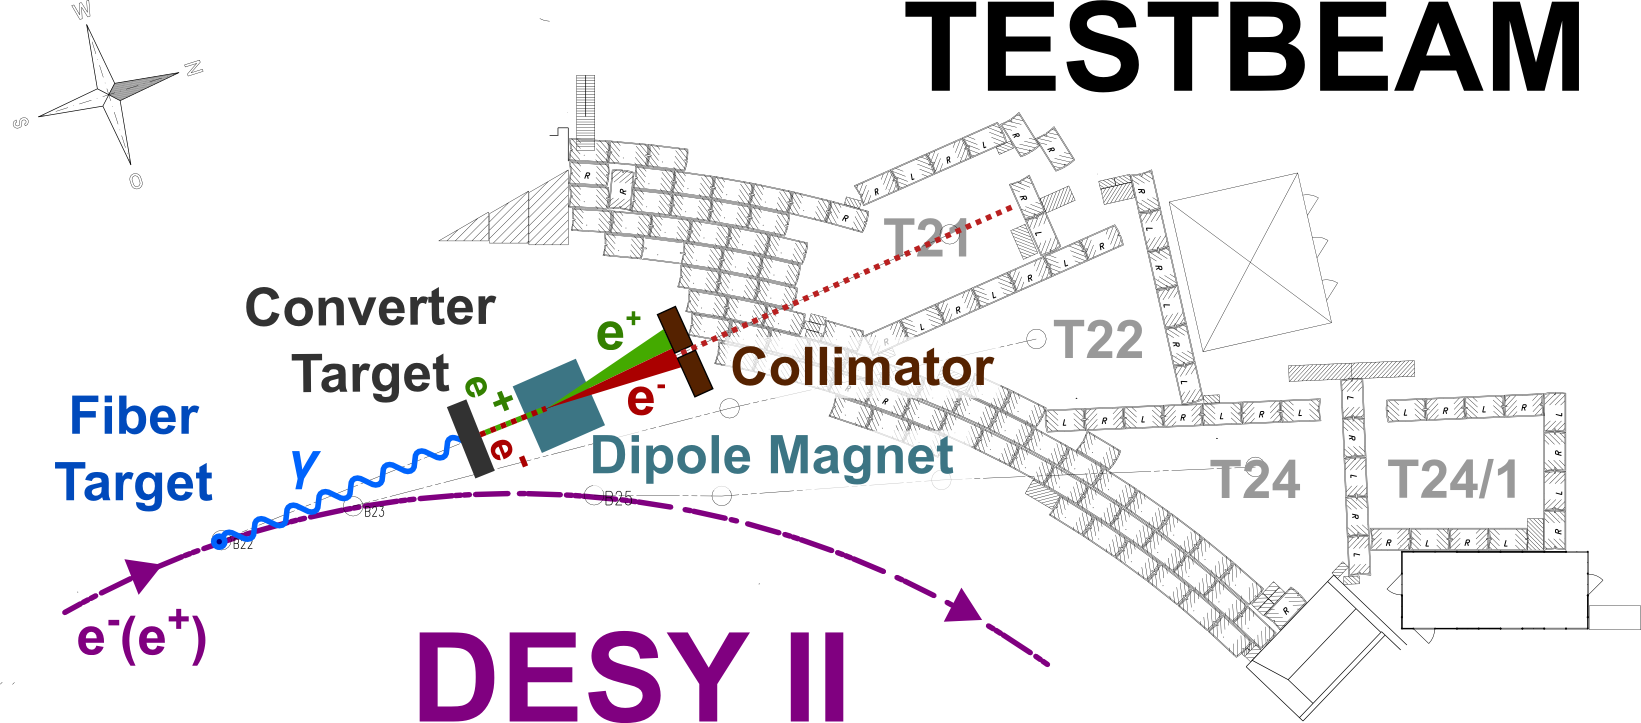
\includegraphics[width = 0.8\textwidth]{Pictures/X0/desy_tb-sketch.png}
      \caption{Schematic layout of the DESY-II test beam facility \cite{DESYII}.}
      \label{fig:desyTb-sketch}
    \end{figure}

    To generate the beam delivered in the Hall 26, a graphite fiber target is placed inside the beam pipe.
    While the electrons are hitting the target, they lose energy and emit bremsstrahlung photons.
    The photons travel through the air and hit another target, on which the photons are converted to pairs of electrons and positrons.
    Different targets with different thicknesses are available and this will impact the particles rate.
    One is made of copper, whereas the other one is made of aluminum \cite{ConversionTargets}.
    Then, a dipole magnet bends the particles and spread them according to their energy.
    Afterward, a tungsten collimator cuts away the unwanted particles, those having a too high or too low momentum, before the test beam area.
    A second collimator is located inside the test beam area and it determines the size of the beam spot.
    Figure~\ref{fig:desyTb-sketch} summarises the different steps to generate a beam of electrons or positrons in test beam 21, while the energies and the rates available are displayed in figure~\ref{fig:rateTB21}.
    The energy resolution achieved at DESY test beam reaches $5~\%$.

    \begin{figure}[!h]
      \centering
      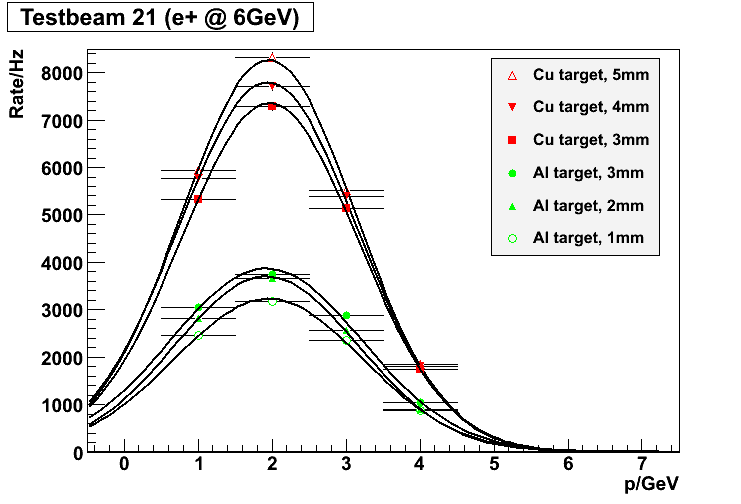
\includegraphics[width = 0.8\textwidth]{Pictures/X0/rate_vs_p_t21.png}
      \caption{Rate for different momentum and with different converter targets \cite{DESYII}.}
      \label{fig:rateTB21}
    \end{figure}

  \section{Analysis}
  \label{sec:X0}

   \subsection{Software analysis chain}

    The analysis of the test beam data is performed with EUTelescope \cite{Eutel}\cite{Jansen}.
    It is based on the MARLIN framework, which is a part of the ILCSOFT (see~\ref{subsec:ILCSOFT} for more details about the ILCSOFT package).
    The software is used to convert the data into the LCIO format and to perform clustering search, alignment and final analysis.
    Each step of the analysis is driven by a dedicated processor and is described in figure~\ref{fig:eutel-strategy}.
    
    \begin{figure}[!h]
      \centering
      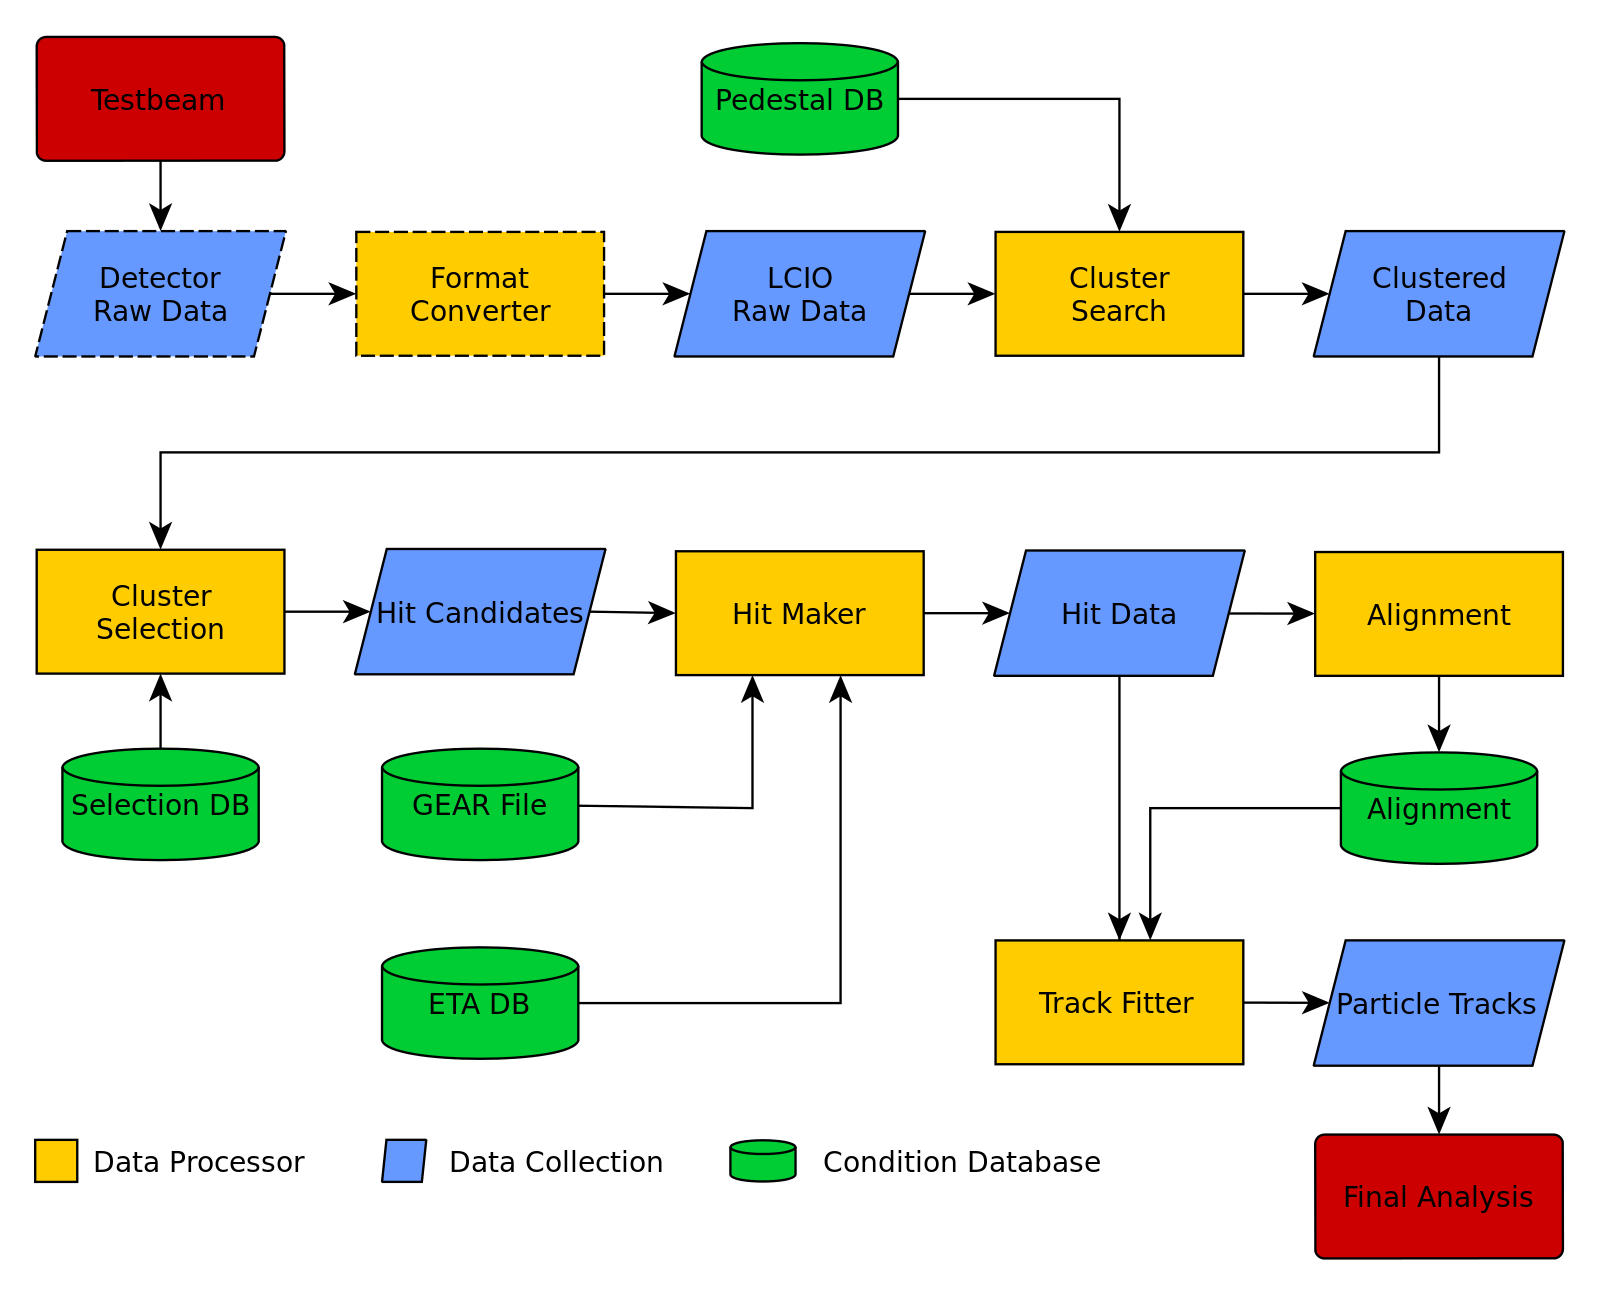
\includegraphics[width = \textwidth]{Pictures/X0/eutel-strategy.png}
      \caption{Flow-chart of the analysis strategy by using EUTelescope \cite{EUTelFlowChart}.}
      \label{fig:eutel-strategy}
    \end{figure}

    A first processor is used to convert the raw data files acquired during the test beam into the LCIO format.
    The new file created contains the pixel number which fired in a given event, along with the sensor number.
    During the conversion, a hot pixel search is done to remove the noisy pixels from the list of hits.
    A pixel is considered noisy if its firing frequency is above a threshold value determined by the user (typically the cut value is between $0.001~\rm{and}~0.003~\%$).
    The noisy pixels correspond to defective raw or column or single pixels always sending information (see section~\ref{sec:noiseMeasurements}).
    Then, a cluster algorithm forms clusters from adjacent fired pixels in a row and/or column.
    Afterward, the hit candidates are defined with a centre-of-gravity method and the position of the hit is determined in the telescope frame and in the sensor frame using the alignment constant.

    Although the alignment procedure looks like the one presented in chapter~\ref{chap:deformation}, the procedure used with EUTelescope is slightly different.
    The alignment is performed with \gls{GBL} and MILLEPEDE-II \cite{MPII}.
    In the case of a complete telescope (six planes), the tracks are built from the reconstruction of triplets in the upstream and downstream telescope planes.
    Firstly, a hit candidate from the outer plane is extrapolated by a horizontal straight line to the inner plane of one arm.
    Then, a triplet is formed if there is a matching between the middle plane of the arm and the doublet built.
    This is done on the two arms and a criterion ensures that two triplets are coming from the same track if the distance between the two extrapolated triplets at the middle $z$-position of the telescope is below a cut value.
    This was set to $10~\rm{\mu m}$.
    \gls{GBL} forms a track from the six hits belonging to the matching triplets.
    The track candidates are then passed to MILLEPEDE-II, which determines the shift and the rotation to apply for aligning the sensors.
    This method is applied a couple of times, until the precision of the alignment reaches a submicron order.

    Nevertheless, due to the set-up used during the test beam and a limitation in EUTelescope on the number of telescope planes and the ID used, the alignment did not work for practical reasons.
    The number of telescope planes is hard-coded to be six and the sensor IDs in the range $[0; 5]$ are reserved for the telescope. 
    Here, the IDs $0$ and $1$ are used for \gls{PLUME} and the others for the telescope.
    Thus, a modification has to be applied to remap the sensor IDs. 
    Although this solution can work and \gls{GBL} uses only the $z$ ordering information is used to create the tracks, EUTelescope is waiting for six hits.
      
    %Another problem occurs during the analysis of the data. 
    %EUTelescope is not able to handle the particular configuration used during the test beam.
    %The number of telescope sensors are hard-coded, as well as the expected sensor ID.
    %Besides, the combination of \gls{GBL} and MILLEPEDE-II inside EUTelescope did not work.
    %The use of a different software reading the hitmaker file created by EUTelescope has permitted to overcome this problem and to perform the alignment and analysis 

    Thankfully, a prototype software developed by Claus \textsc{Kleinwort} has permitted to perform the alignment and finish the analysis. 
    It is based on \gls{GBL} and MILLEPEDE-II and reads the hit information created by the hitmaker processor of EUTelescope. 
    The modularity of the software allows to select the desire number of telescope planes.
    In the case of only four telescope planes, the triplets method is not used and tracks are formed only with doublets.
    Then, the track's information are feed to MILLEPEDE-II, which calculates the residuals of the tracks on each sensor and attempts to shift the position and rotate the sensors to minimise the east square fit function of these tracks.
    MILLEPEDE-II creates an output file with theses informations and a script update the GEAR file with the new position and orientation of each planes.

    \todo{Alignment plots}

   \subsection{Measurement of the radiation length}

     \subsubsection{Theoretical estimation}

     The theoretical estimation of \gls{PLUME} material budget was already discussed in chapter~\ref{chap:vxd}.
     The value defined in this chapter was a weighted radiation length, which takes into account the passive component and the insensitive areas.
     For the measurement done here, only the region over a sensitive surface is studied.
     There is no passive component and the beam is travelling through:
     
     \begin{itemize}
       \item Two \gls{MIMOSA}-26 sensors thinned down to $\sim 50~\rm{\mu m}$ and a material budget of $\left. \frac{x}{X_0} \right|_{\rm{Mi26}} \sim 0.053~\%~\rm{X_{0}}$,
       \item Four layers of glue (sensor/flex interface and flex/stiffener interface) with an estimated radiation length: $\left. \frac{x}{X_0} \right|_{\rm{Glue}} \sim 0.01~\%~\rm{X_0}$,
       \item Stiffener made of $8~\%$ density \gls{SiC} with a thickness of $\sim 2~\rm{mm}$ and radiation length: $\left. \frac{x}{X_0} \right|_{\rm{SiC}} ~\sim 0.184~\%~\rm{X_{0}}$,
       \item Two flex-cables made of two copper layers insulated with three layers of Kapton:
       \begin{itemize}
         \item Material budget for $\sim 50~\rm{\mu m}$ of Kapton: $\left. \frac{x}{X_0} \right|_{\rm{Kapton}} \sim 0.014~\%~\rm{X_{0}}$,
         \item Material budget for $\sim 14~\rm{\mu m}$ of Copper: $\left. \frac{x}{X_0} \right|_{\rm{Cu}} \sim 0.084~\%~\rm{X_{0}}$.
       \end{itemize}
     \end{itemize}

     It is assumed that the copper layers have a fill factor between $25~\%$ and $30~\%$.
     Hence, the flex-cable material budget is: $\left. \frac{x}{X_0} \right|_{\rm{Flex}} \sim 0.084~-~0.092~\%~\rm{X_0}$, leading to a total radiation length of:

     \begin{equation}
       \begin{array}{lcl}
         \left. \frac{x}{X_0} \right|_{\rm{PLUME}} & = & 2 \times \left( \left. \frac{x}{X_0} \right|_{\rm{Mi26}} + \left. \frac{x}{X_0} \right|_{\rm{Flex}} + 2 \times \left. \frac{x}{X_0} \right|_{\rm{Glue}}\right) + \left. \frac{x}{X_0} \right|_{\rm{SiC}}, \\
         \\
         & \simeq & 0.498~-~0.515~\%~\rm{X_0}.
       \end{array}
       \label{eq:X0_theory}
     \end{equation}

     Hence, the material budget expected is between $0.498~\%~\rm{X_0}$ and $0.515~\%~\rm{X_0}$.

     \subsubsection{Kink angle measurement}

   To measure the kink angle of the tracks, the four telescope planes, as well as the two \gls{PLUME} sensors are used.
   So, the hit information provided by \gls{PLUME} are exploited to create tracks by using the triplets method.
   The deviation from the incoming tracks and the outgoing ones (after the \gls{PLUME} ladder) is measured with \gls{GBL}, which provides information for $xz$ and $yz$-angles.
   Figure~\ref{fig:kinkAngle5GeV} shows the distribution of the kink angle fitted by a Gaussian for an energy of $5~\rm{GeV}$ and without a fiducial cut on a particular region of interest.
   For small deflection angles, the distribution is roughly Gaussian with larger tails than expected for a Gaussian distribution \cite{Agashe:2014kda}.
   Therefore, the fit is performed in a range corresponding to the standard deviation of the distribution.
   %Therefore, the fit is performed only on the $1 \sigma$ range of the distribution.
   To obtain $\theta_0$, the width of the kink angle $\rm{\sigma_{kink~angle}}$ has to be corrected by the mean value of the kink angle fit $<\rm{kink~angle}>$:
   
   \begin{equation}
     \theta_0 = \sqrt{\rm{\sigma_{kink~angle}}^2 - <\rm{kink~angle}>}.
     \label{eq:kink}
   \end{equation}
   
   From the equation~\ref{eq:theta0} and by injecting $\theta_0$ defined in equation~\ref{eq:kink}, the radiation length $\frac{x}{X_0}$ is then:
   
   \begin{equation}
     \frac{x}{X_{0}} = \left( \frac{\sqrt{\rm{\sigma_{kink~angle}}^2 - <\rm{kink~angle}>} \cdot p}{13.6~\rm{(MeV)}} \right)^{\frac{1}{0.555}}.
   \end{equation}

   The kink angle measured at $5~\rm{GeV}$ is $\sim 1.95 \cdot 10^{-4}~\rm{rad}$, leading to a radiation length of $\sim 0.58~\%~\rm{X_0}$, which is over the estimated calculation.
   
   \begin{figure}[!h]
     \centering
     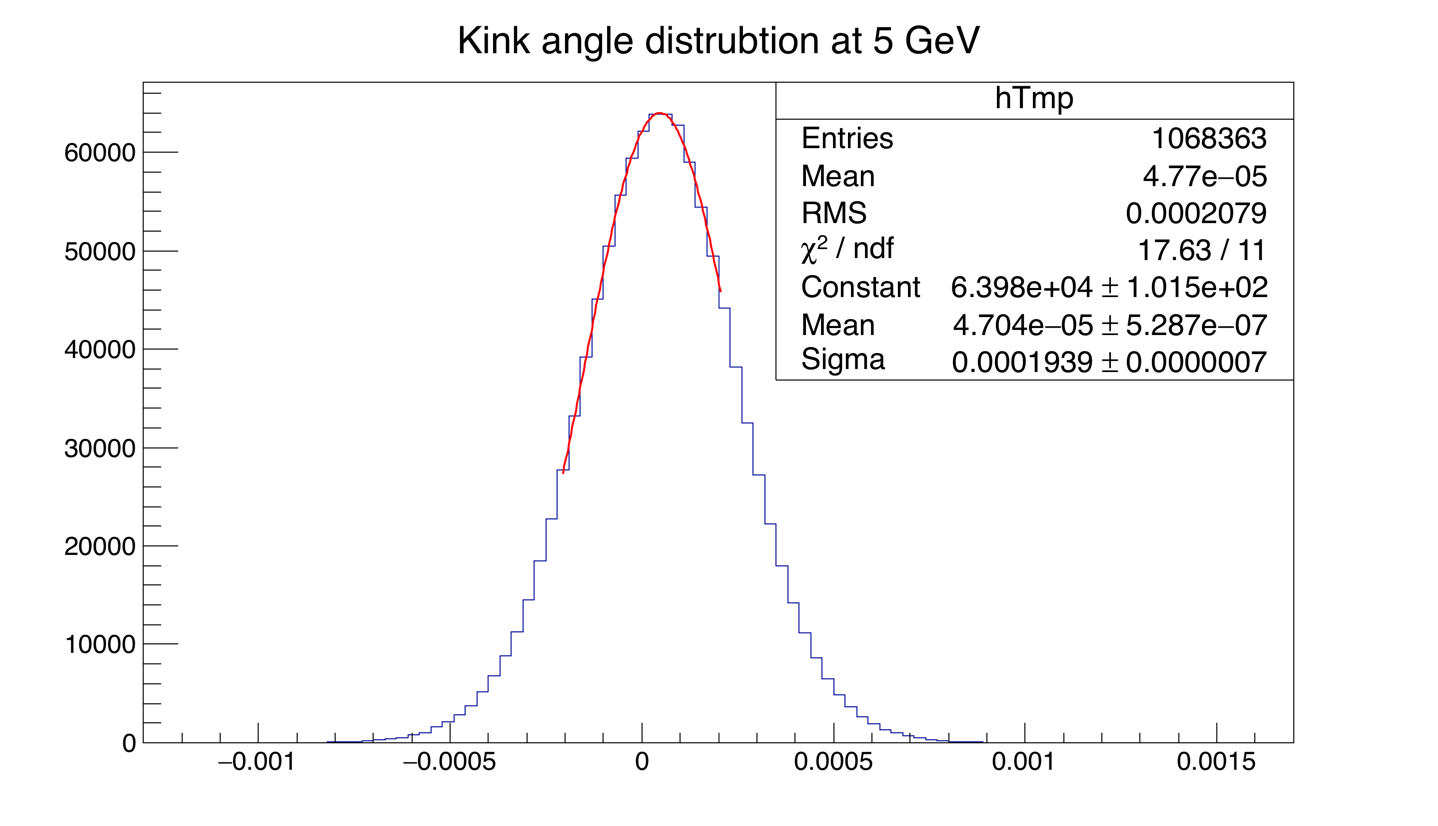
\includegraphics[width = \textwidth]{Pictures/X0/kinkAngle5GeV_2.png}
     \caption{Distribution of the kink angle given by GBL for an energy of $5~\rm{GeV}$ without any fiducial cut. The asymmetric fit arises from a wrong alignment procedure.}
     \label{fig:kinkAngle5GeV}
   \end{figure} 

   \begin{figure}[!p]
     \centering
     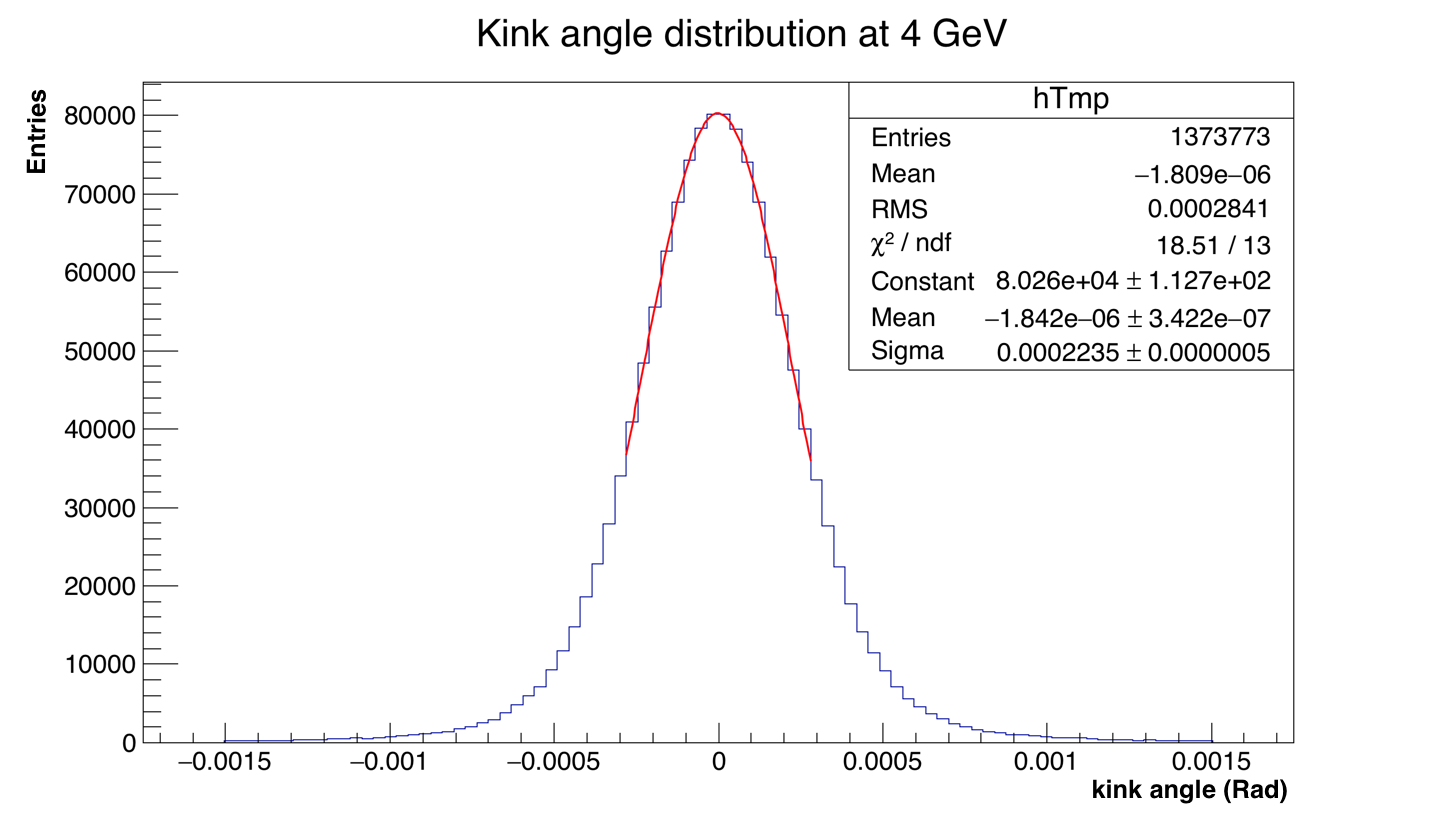
\includegraphics[width = \textwidth]{Pictures/X0/kinkAngle4GeV.png}
     \caption{Distribution of the kink angle given by GBL for an energy of $4~\rm{GeV}$ without any fiducial cut.}
     \label{fig:kinkAngle4GeV}
   \end{figure} 

   \begin{figure}[!p]
     \centering
     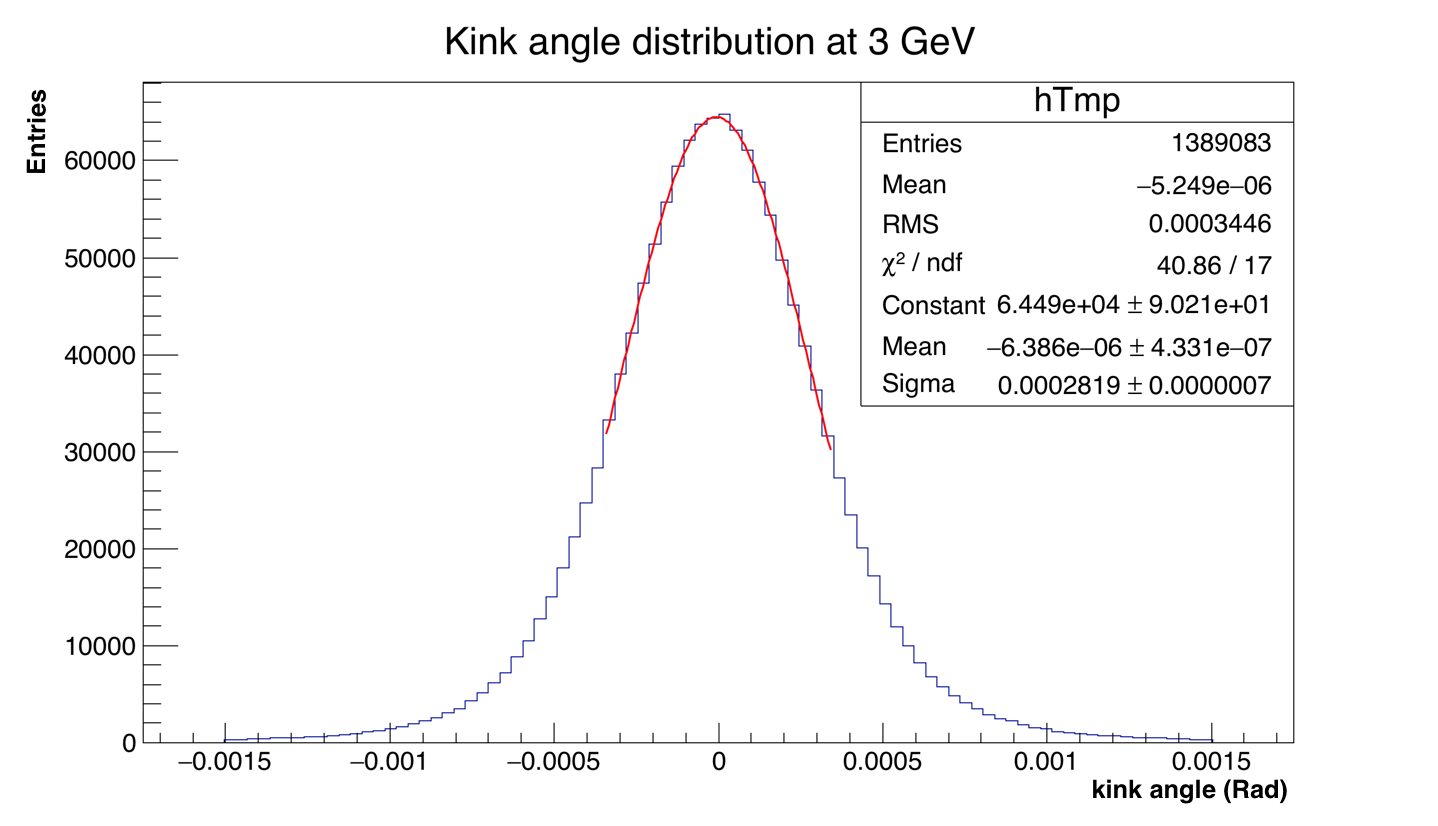
\includegraphics[width = \textwidth]{Pictures/X0/kinkAngle3GeV.png}
     \caption{Distribution of the kink angle given by GBL for an energy of $3~\rm{GeV}$ without any fiducial cut.}
     \label{fig:kinkAngle3GeV}
   \end{figure} 

   \begin{figure}[!p]
     \centering
     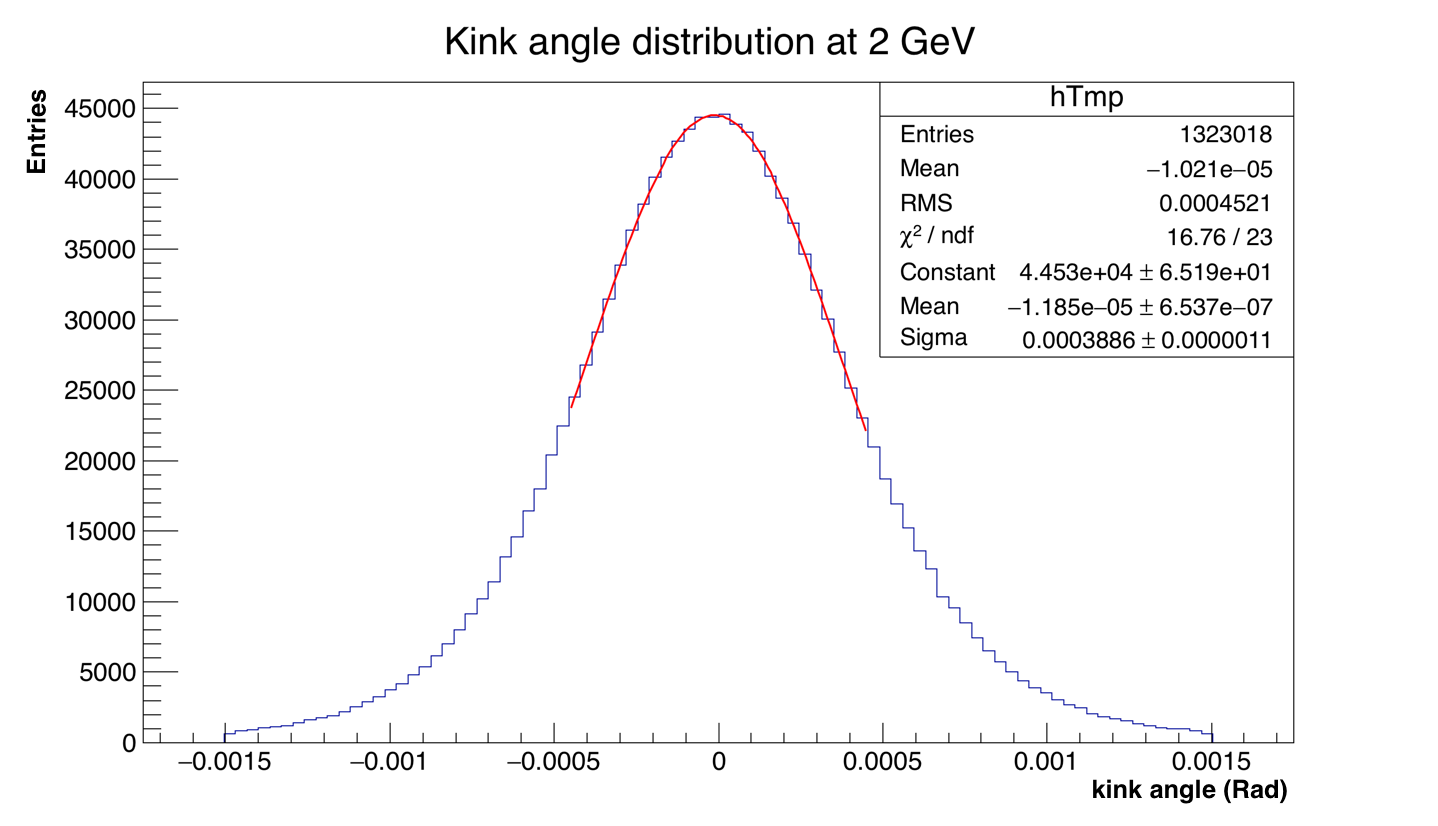
\includegraphics[width = \textwidth]{Pictures/X0/kinkAngle2GeV.png}
     \caption{Distribution of the kink angle given by GBL for an energy of $2~\rm{GeV}$ without any fiducial cut.}
     \label{fig:kinkAngle2GeV}
   \end{figure} 

   \begin{figure}[!p]
     \centering
     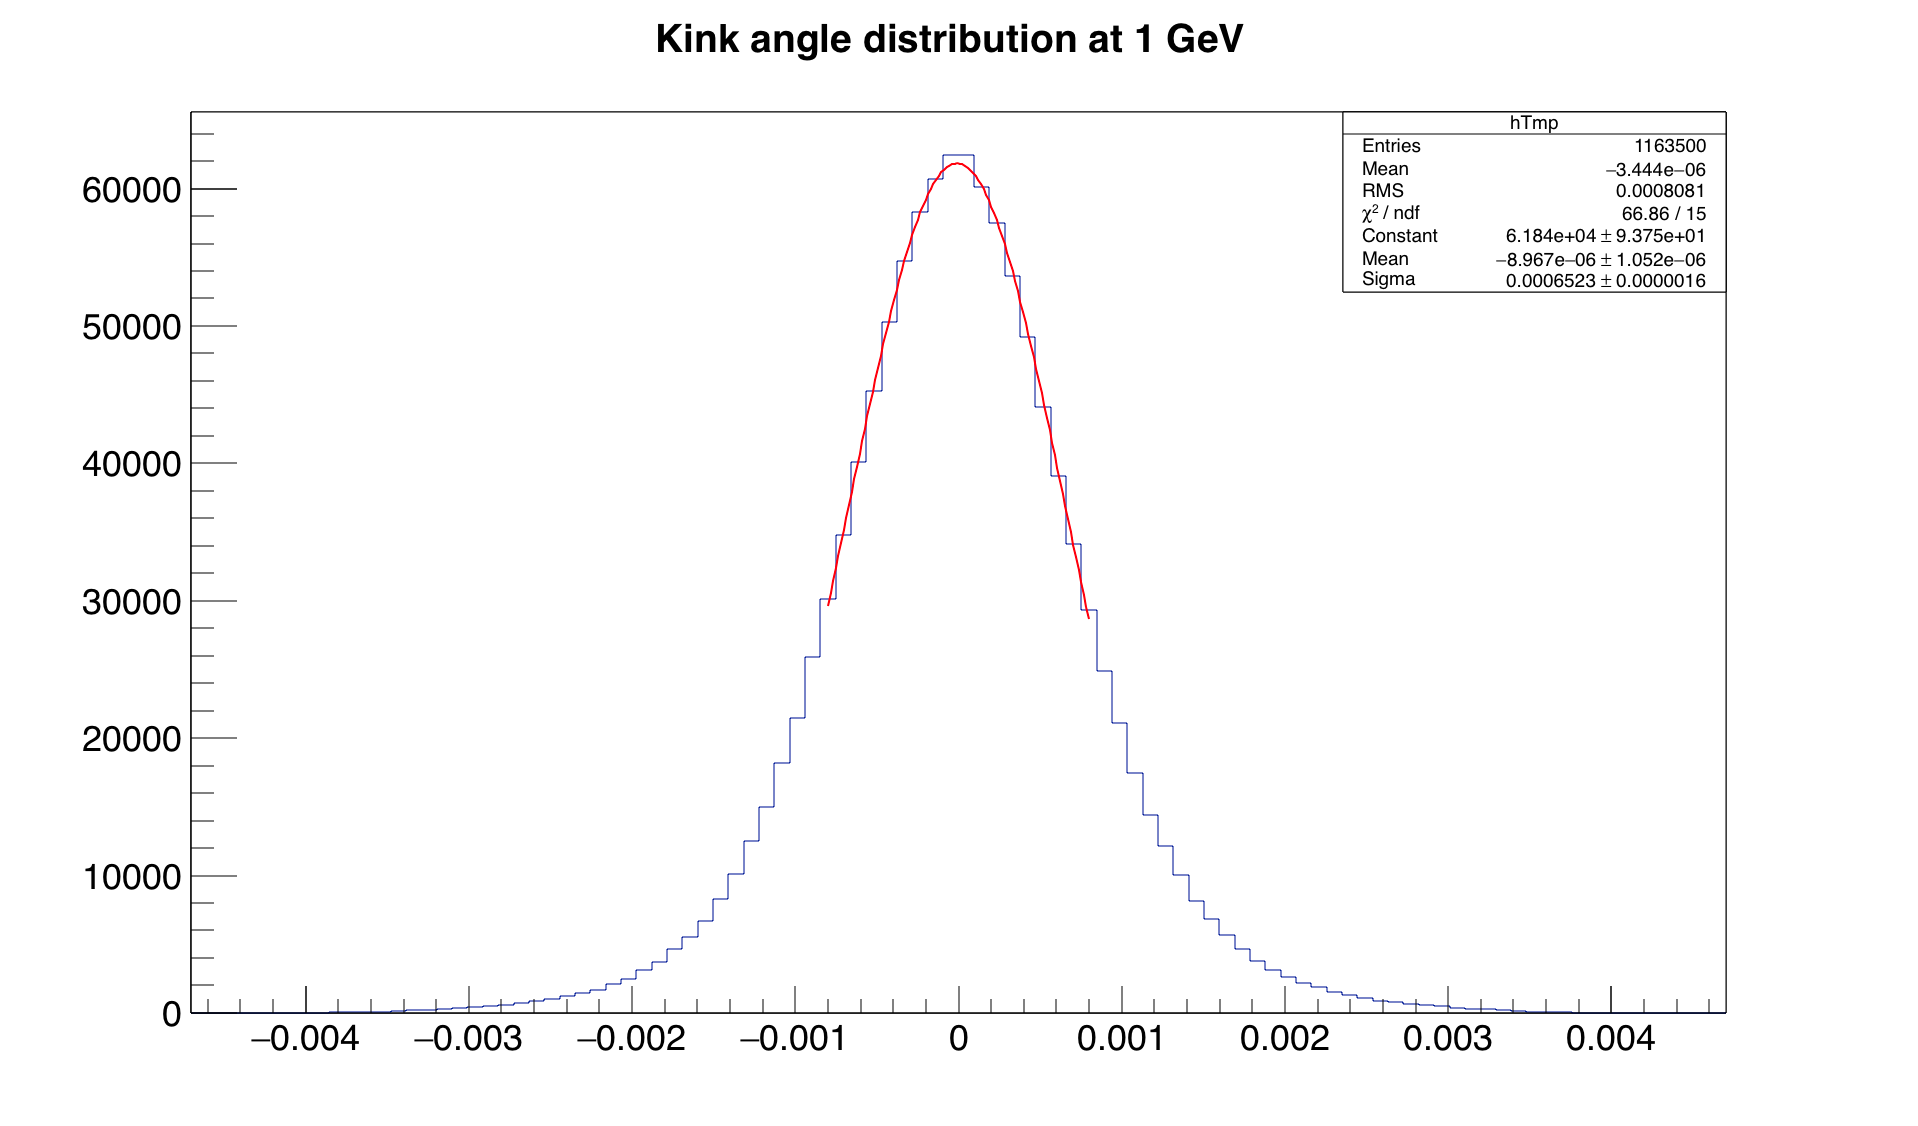
\includegraphics[width = \textwidth]{Pictures/X0/kinkAngle1GeV.png}
     \caption{Distribution of the kink angle given by GBL for an energy of $1~\rm{GeV}$ without any fiducial cut.}
     \label{fig:kinkAngle1GeV}
   \end{figure} 

   This procedure has been repeated to the runs between $1$ and $4~\rm{GeV}$ (see figures~\ref{fig:kinkAngle4GeV} to~\ref{fig:kinkAngle1GeV}) and the results of the measured kink angles as a function of the beam momentum are represented on figure~\ref{fig:theta0vsP_all}. 
   The uncertainty on the momentum is $5~\%$ and is the uncertainty determined at the DESY test beam facility, while the uncertainty used for the kink angle is extracted from the fit procedure corrected by the $\chi^2 / \rm{NDF}$ measured.
   The plot is then fitted with the Highland formula from equation~\ref{eq:theta0}, on which the radiation length is a free parameter.
   Two points ($1$ and $5~\rm{GeV}$) are outside the trend and the $\chi^2 /~\rm{N.D.F}$ measured is bigger than $1$.
   Table~\ref{tab:theta0Calcultation} summarises the expected $\theta_0$ for a radiation length of $0.5~\%~\rm{X_0}$ and compare this results to the measured $\theta_0$.

   \begin{table}
     \centering
     \begin{tabular}{c c c c}
        \hline %----------------------------
        Energy (GeV)	& $\left. \theta_0\right|_{\rm{expected}}~(\rm{rad})$ & $\left. \theta_0\right|_{\rm{measured}}~(\rm{rad})$ \tabularnewline
        \hline %----------------------------
        \hline %----------------------------

        	1	  &		$7.186 \cdot 10^{-4}$	  &		$5.740 \cdot 10^{-4} \pm 2.783 \cdot 10^{-6}$	      \tabularnewline
        	2		&		$3.592 \cdot 10^{-4}$	  &		$3.337 \cdot 10^{-4} \pm 7.764 \cdot 10^{-7}$	      \tabularnewline
        	3		&		$2.395 \cdot 10^{-4}$	  &		$2.380 \cdot 10^{-4} \pm 1.610 \cdot 10^{-6}$       \tabularnewline
        	4		&		$1.796 \cdot 10^{-4}$	  &	  $1.821 \cdot 10^{-4} \pm 7.483 \cdot 10^{-7}$       \tabularnewline
        	5		&		$1.437 \cdot 10^{-4}$   &		$1.549 \cdot 10^{-4} \pm 1.136 \cdot 10^{-4}$	      \tabularnewline
        \hline %----------------------------
     
     \end{tabular}
     \caption{Determination of $\left. \theta_0\right|_{\rm{expected}}$ for a material budget of $0.5~\%~\rm{X_0}$ and comparison to $\left. \theta_0\right|_{\rm{measured}}$.}
     \label{tab:theta0Calcultation}
   \end{table}

   \begin{figure}[!h]
     \centering
     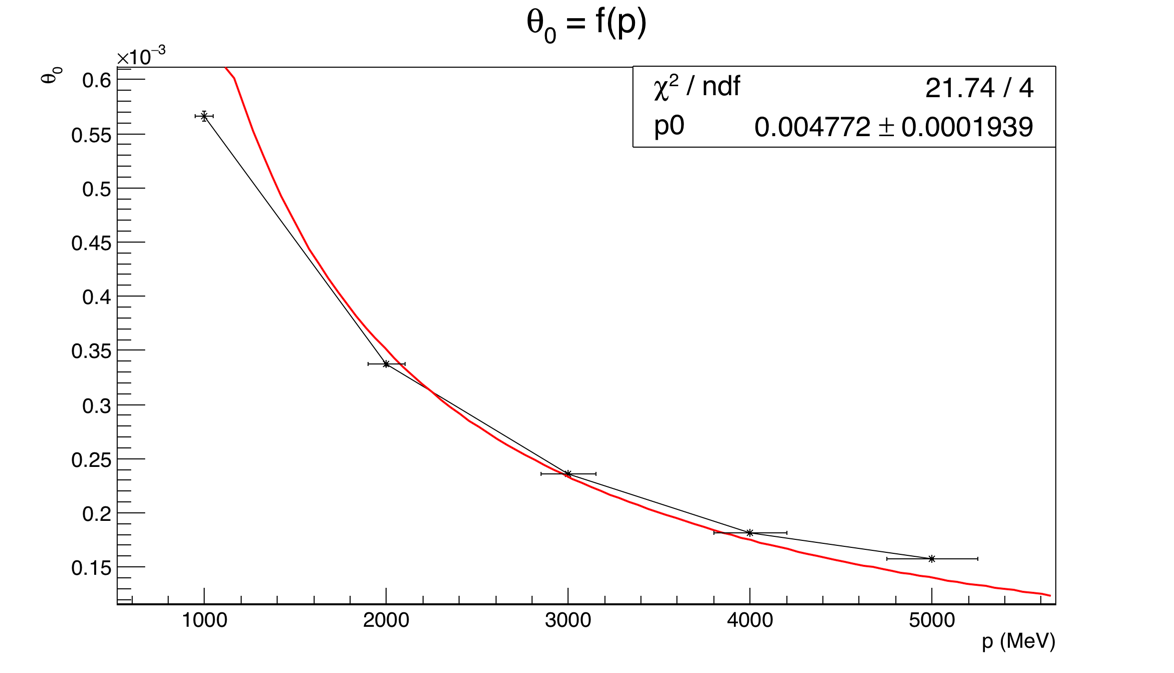
\includegraphics[width = \textwidth]{Pictures/X0/theta0VsP_all.png}
     %\caption{Extrapolation of the measured radiation length with a fit between 1 and 5 GeV.}
     \caption{Dependence of the measured standard deviation of the kink angle with the energy, over the full range of the energies used. Superimposed is a fit using the Highland formula where the radiation length is left as a free parameter.}
     \label{fig:theta0vsP_all}
   \end{figure}

   The alignment of the $1~\rm{GeV}$ runs are complicated to perform.
   At this energy, the electrons are more sensitive to the multiple scattering in the air and inside the detectors.
   At $5~\rm{GeV}$, the electrons suffer less from the multiple scattering but the alignment procedure did not work well. 
   On figure~\ref{fig:kinkAngle5GeV}, the distribution of the kink angle is not centered and the reason of this offset comes from a wrong alignment.
   For the rest of the study, this two measurements are excluded to determine the radiation length, as seen on figure~\ref{fig:theta0vsP_2-4}.
   The radiation length measured is then $0.47 \pm 0.02~\%~\rm{X_0}$, smaller than the expected calculation.
   The determination of the material budget is done here without taking into account the complete ladder.
   The \gls{PLUME} sensors are used for tracking and measuring the kink angle.
   As the signal is considered to be created in the middle of the epitaxial layer, only one part of the \gls{MIMOSA}-26 is included in the calculation.
   The thickness of the different \gls{MIMOSA}-26 layers are the followings:
   
   \begin{itemize}
     \item Electronics layer: $\sim 6~\rm{\mu m}$,
     \item Epitaxial layer: $\sim 14~\rm{\mu m}$,
     \item Bulk: $\sim 30~\rm{\mu m}$.
   \end{itemize}

   The sensors are thinned down to $50 \pm 2~\rm{\mu m}$, but only $\sim 37~\rm{\mu m}$ of silicon are taken into account during the calculation.
   In total, $0.028~\%~\rm{X_{0}}$ are missing in the calculation.
   
   \begin{figure}[!h]
     \centering
     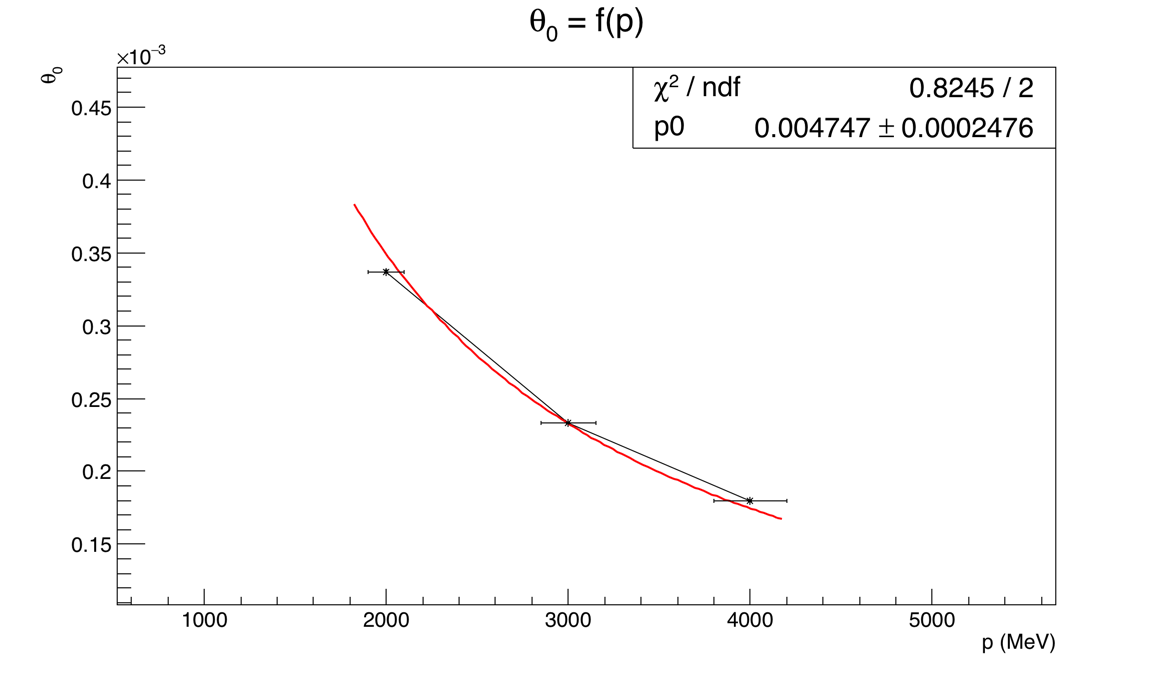
\includegraphics[width = \textwidth]{Pictures/X0/theta0VsP_2-4GeV.png}
     %\caption{Extrapolation of the measured radiation length in the range 2 to 4 GeV.}
     \caption{Extrapolation of the kink angle with the energy, over a restricted range of the energies used.
     Superimposed is a fit using the Highland formula, where the radiation length is left as a free parameter.}
     \label{fig:theta0vsP_2-4}
   \end{figure}

   To insure that the measurement is correct, the different radiation lengths measured are plotted as a function of the momentum (see figure~\ref{fig:X0vsP}).
   Although the fit shows a dependency on the momentum, the error on the second polynom is larger than the value determined by the fit.
   The different radiation lengths determined at different momentum are of the same order and this is consistent with the definition of the material budget.


   %The sensors are thinned down to $50 \pm 2~\rm{\mu m}$ and the signal is considered to be created in the middle of the epitaxial layer. 
   %Thus, only $\sim 37~\rm{\mu m}$ for a sensor is taken into account during the measurement, leading to approximately $0.028~\%~\rm{X_{0}}$ less than the theoretical value.
   %By adding the $0.028~\%$ missing, the total radiation length over a sensitive surface is $0.498~\%$, the material budget determined for a flex with a $25~\%$ fill factor (see equation~\ref{eq:X0_theory}).

   \begin{figure}
     \centering
     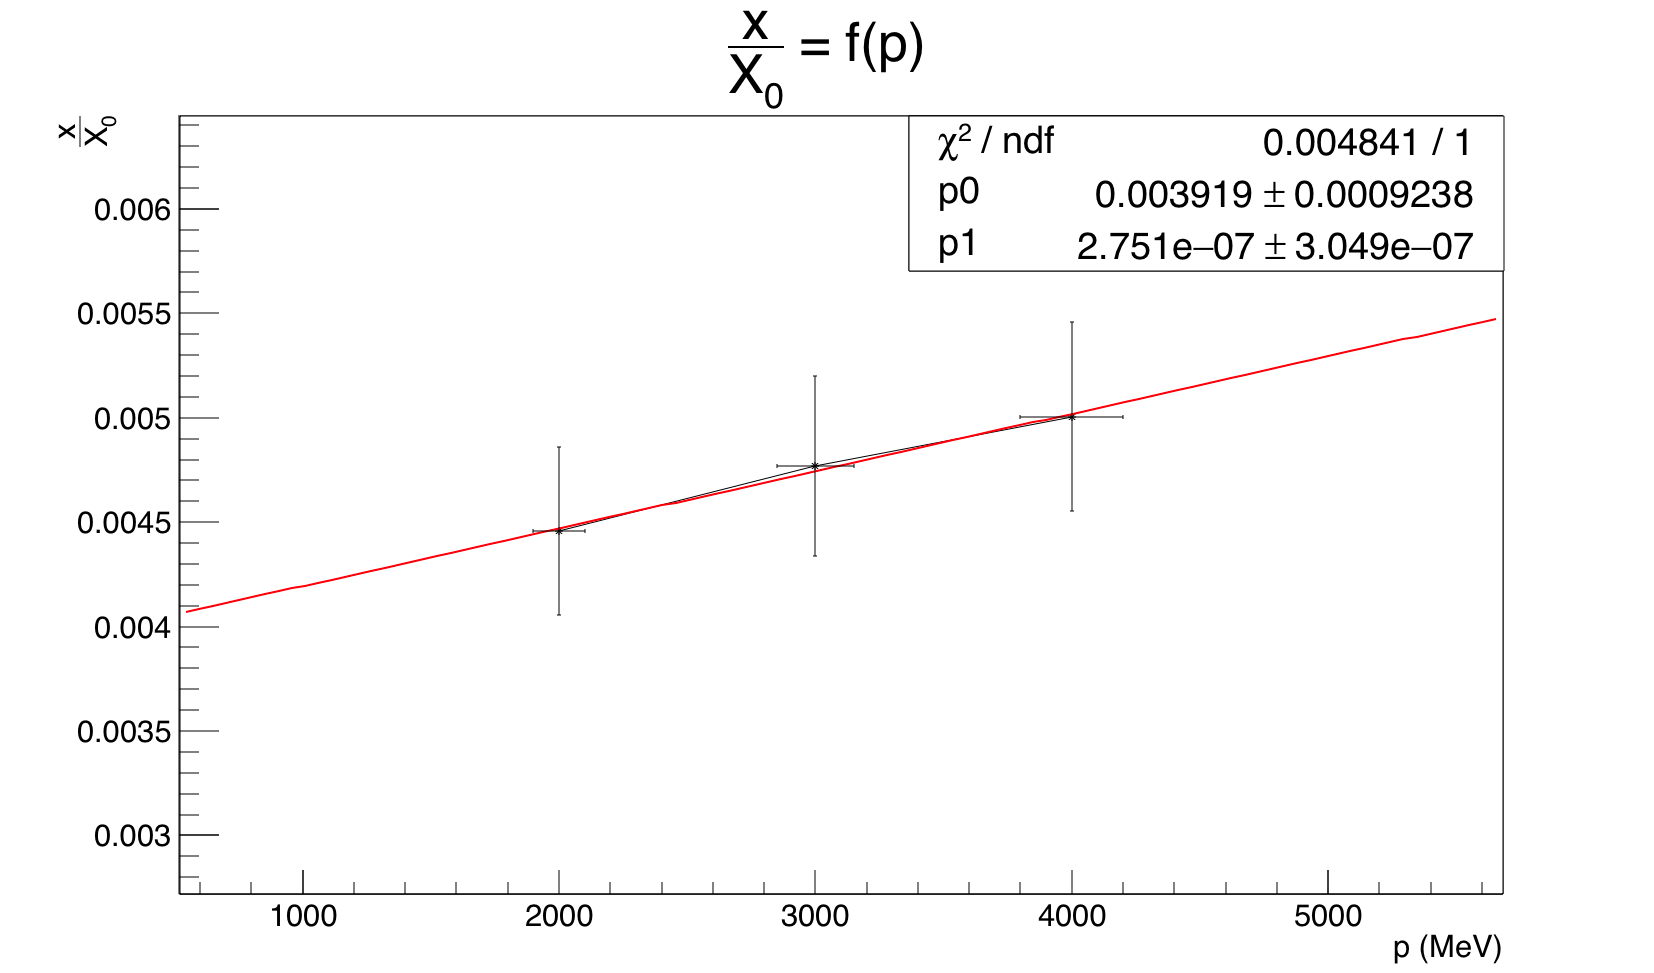
\includegraphics[width =\textwidth]{Pictures/X0/radiationLength_2-4GeV.png}
     \caption{Measured radiation lentgh $\frac{x}{X_0}$ as a function of the momentum $p$.}
     \label{fig:X0vsP}
   \end{figure}

  \section{Conclusions}

%  The preparation of the test beam, as well as the data taking were a long and stressful period.
%  Although everything were prepared as mush as possible to avoid any problem during the test beam, a broken component on the power distribution board has disturbed the data taking for two days.
%  One \gls{PLUME} module was not recording data anymore but was still sending \textit{header} and \textit{trailer}.
%  Fortunately, after replacing the broken component, the ladder was working normally, but a shift on the thresholds has appeared.
%  By characterising again the ladder, it has been possible to determine which thresholds were really applied. 
%  Nevertheless, it is likely that some data could have been corrupted and this is under investigation.

  %Another problem occurs during the analysis of the data. 
  %EUTelescope is not able to handle the particular configuration used during the test beam.
  %The number of telescope sensors are hard-coded, as well as the expected sensor ID.
  %Besides, the combination of \gls{GBL} and MILLEPEDE-II inside EUTelescope did not work.
  %The use of a different software reading the hitmaker file created by EUTelescope has permitted to overcome this problem and to perform the alignment and analysis 

  The radiation length measurement of the \gls{PLUME} ladder was performed for the first time with a dedicated setup placed in beam.
  The first results obtained to determine the material budget, which gives a radiation length of $\left. \frac{x}{X_0} \right|_{\rm{measured}} \simeq 0.47 \pm 0.02~\%~\rm{X_0}$ are confirming the theoretical calculation of $\left. \frac{x}{X_0}\right|_{\rm{theoretical}} \simeq 0.498~~\%~\rm{X_0}$ for a flex with a fill factor of $25~\%$.
  The origin of the shifts on the measured radiation length at $1$ and $5~\rm{GeV}$ has to be investigated.
  In both cases, the alignment has to be done again.
  Another solution consists to perform a calibration run with a known material to apply then a correction on the radiation length measurement for \gls{PLUME}.

